%%%%%%%%%%%%%%%%%%%%%%%%%%%%%%%%%%%%%%%%%%%%%%%%%%%%%%%%%%%%%%%%%%%%%%%%%%%%%%%%%%%%%%%%%%%%%%%%%%%%%%%%%%%%%%
%                                                                                                            
%
% ------------------------------------------------------------------------------------------------------------ 
%  @desc        Diploma Thesis Digital Capnometer Module
% ------------------------------------------------------------------------------------------------------------
%               Written by Bastian Großauer
%
% @authors      Bastian Großauer & René Hahn
% 
% @datum        14.01.2022
% @file         DA.tex
%
% @depend       DA_1-4_CAPNO_nf.pdf --------------------------------------------------------------------------
%               DA_5-6_CAPNO_nf.pdf --------------------------------------------------------------------------
%               DA_7-8_CAPNO_nf.pdf --------------------------------------------------------------------------
%
% @comment      Diverse functions and packages only in LuaLaTex available
%               Therfore compile in LuaLaTeX ONLY!!!
%
%
%%%%%%%%%%%%%%%%%%%%%%%%%%%%%%%%%%%%%%%%%%%%%%%%%%%%%%%%%%%%%%%%%%%%%%%%%%%%%%%%%%%%%%%%%%%%%%%%%%%%%%%%%%%%%%               


\documentclass[12pt]{article}

%%%%%%%%%%%%%%%%%%%%%%%%%%%%%%%%%%%%%%%%%%%%%%%%%%% imports %%%%%%%%%%%%%%%%%%%%%%%%%%%%%%%%%%%%%%%%%%%%%%%%%%%

\usepackage{lingmacros}
\usepackage{tree-dvips}
\usepackage{fancyhdr}
\usepackage[utf8]{inputenc}
\usepackage{fontspec}
\usepackage{graphicx}
\usepackage[document]{ragged2e}
\usepackage{xcolor}  
\usepackage{tabto}   
\usepackage{comment} 
\usepackage{pdfpages} 
\usepackage[12pt]{moresize}
\usepackage{lipsum}
\usepackage{titlesec}
\usepackage{geometry}
\usepackage{afterpage}
    \geometry{
                twoside,
                a4paper,
                total={165mm,240mm},                                                    % used text area
                left=22.5mm,                                                            % explanation: https://www.overleaf.com/learn/latex/Page_size_and_margins
                top=30mm,   
            }

\setmainfont{Arial}
\setlength{\headsep}{1.5cm}                                                             % set spce between header and section

% %%%%%%%%%%%%%%%%%%%%%%%%%%%%%%%%%%%%%% Page and Header/Footer Setup %%%%%%%%%%%%%%%%%%%%%%%%%%%%%%%%%%%%%%%%

\pagestyle{fancy}
\fancyhead{}
\fancyfoot{}

\setcounter{secnumdepth}{4}
\setcounter{tocdepth}{4}
\setcounter{secnumdepth}{5}
\setcounter{tocdepth}{5}

\fancyfoot[C]{}
\fancyfoot[RO, LE] {}
\renewcommand{\footrulewidth}{1pt}
\renewcommand{\headrulewidth}{1pt}

\titlespacing\section{0pt}{12pt plus 4pt minus 2pt}{6pt plus 2pt minus 2pt}
\titlespacing\subsection{0pt}{12pt plus 4pt minus 2pt}{6pt plus 2pt minus 2pt}
\titlespacing\subsubsection{0pt}{12pt plus 4pt minus 2pt}{6pt plus 2pt minus 2pt}


%%%%%%%%%%%%%%%%%%%%%%%%%%%%%%%%%%%%%%%%%%%%% Begin of Document %%%%%%%%%%%%%%%%%%%%%%%%%%%%%%%%%%%%%%%%%%%%%

\begin{document}
%                                                                                       % not sure if there should by 1 blank or 2 in 1-4
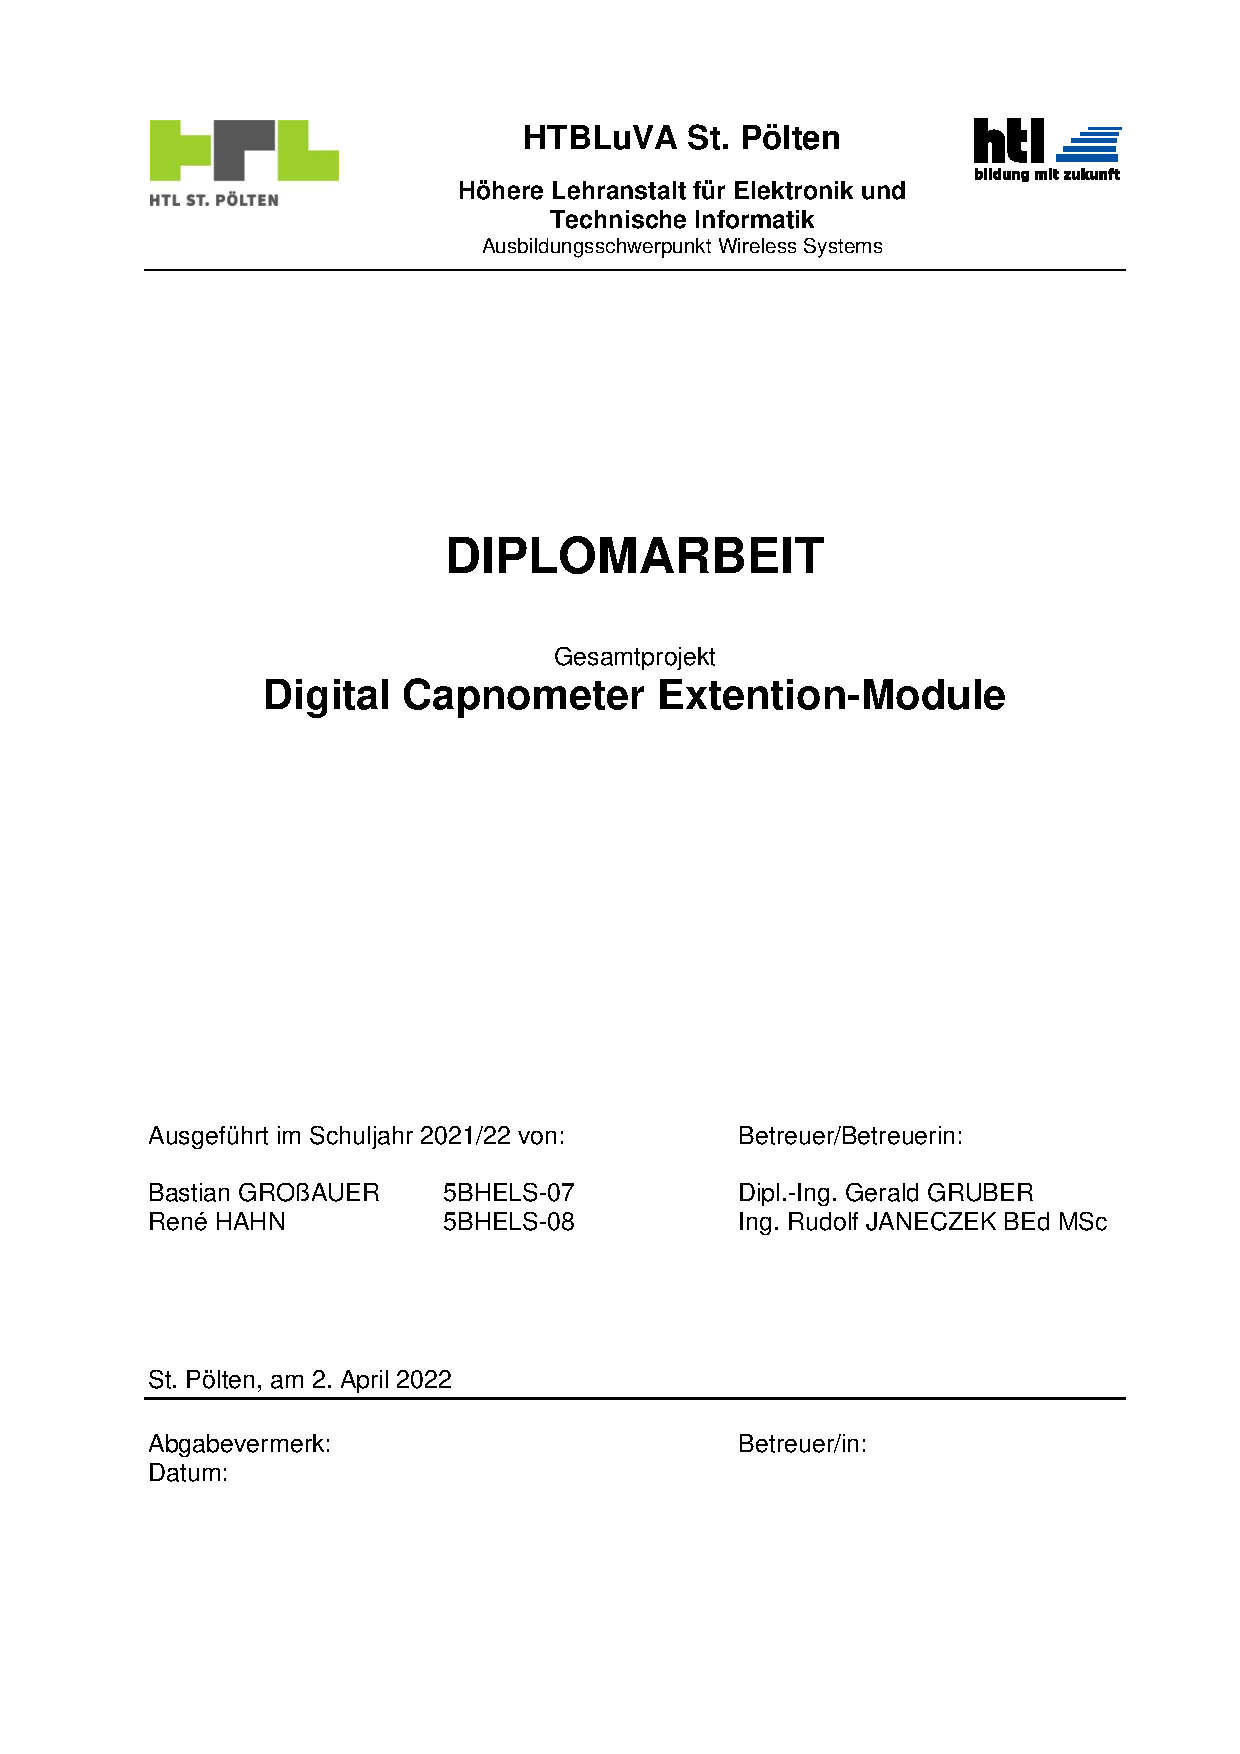
\includepdf[pages={1-3}]{./pdf/DA_1_CAPNO_nf.pdf}                                     % write the initial Document with the 
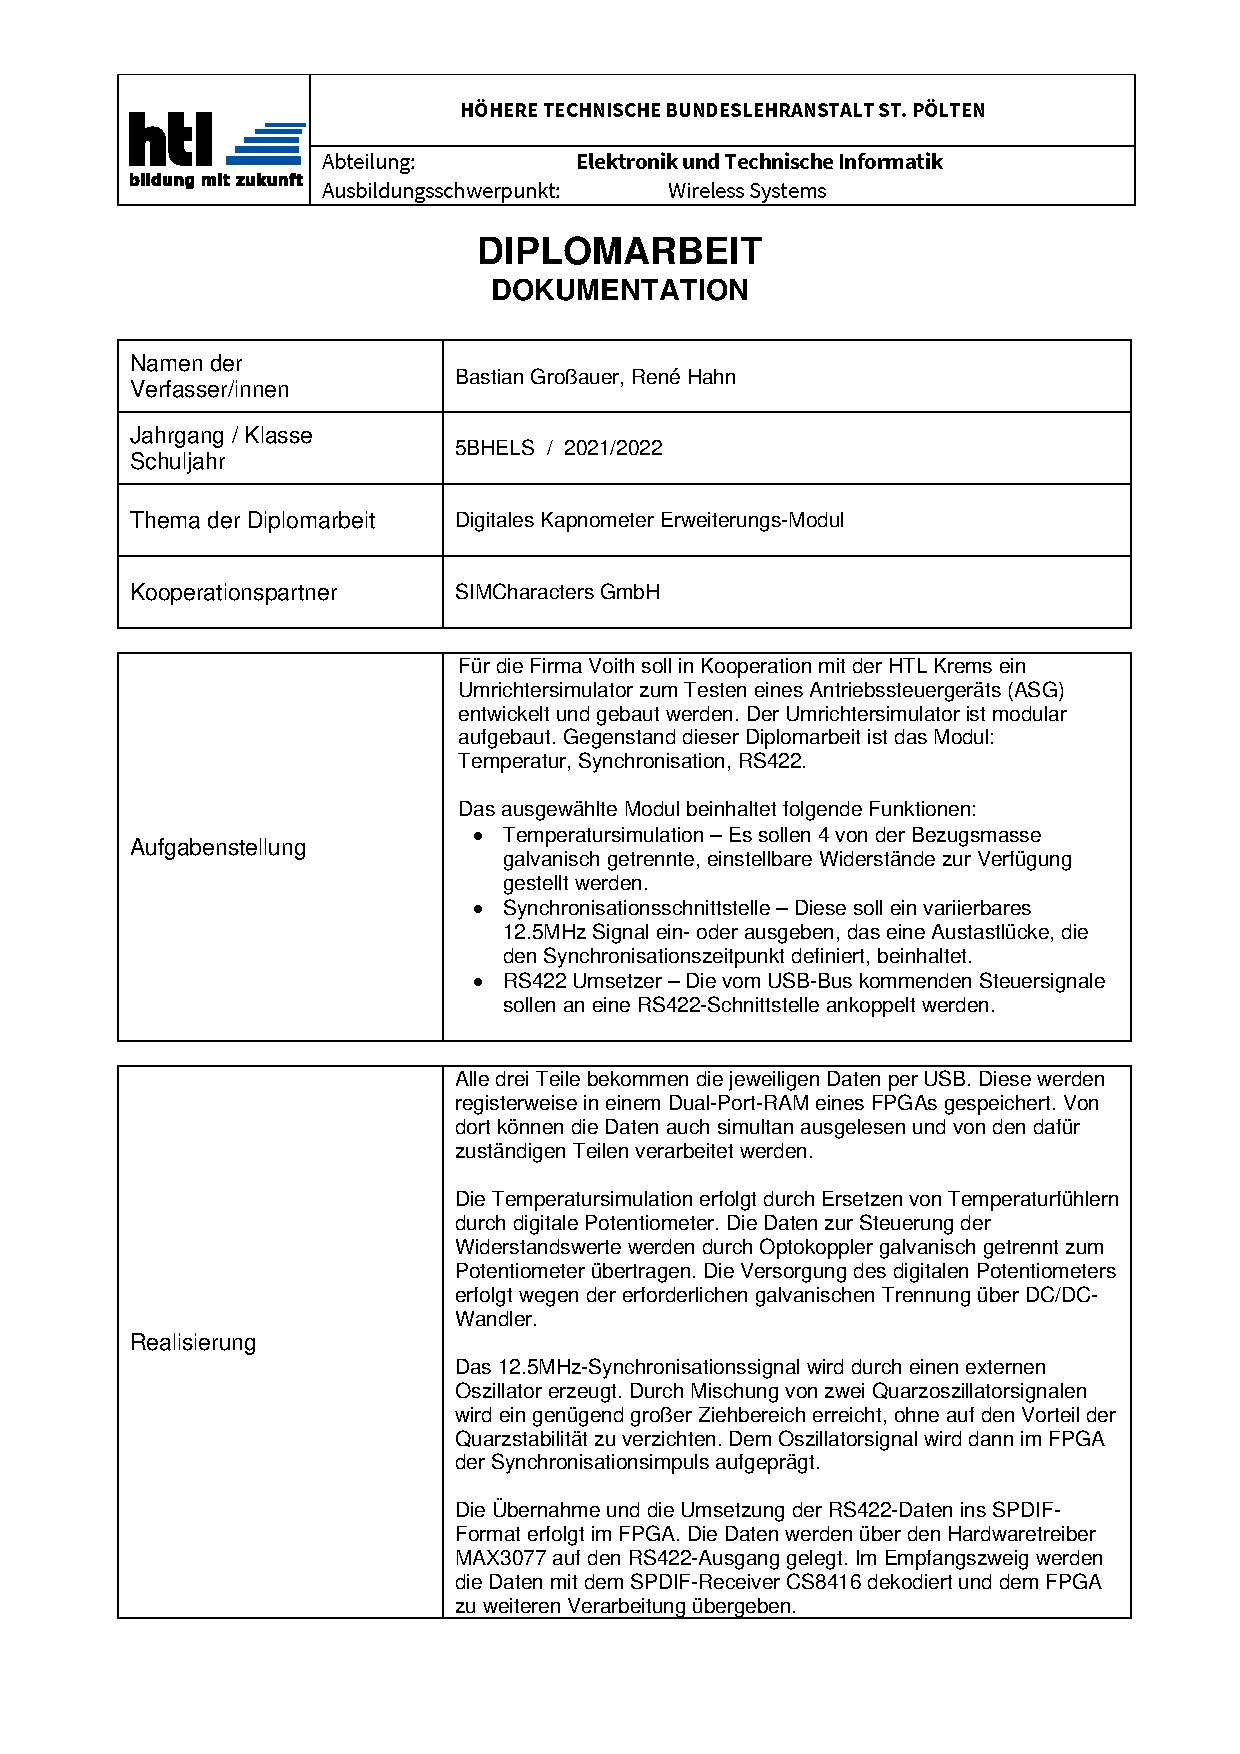
\includepdf[pages={1-2}]{./pdf/DA_2_CAPNO_nf.pdf}                                     % provided templates from sharepoint
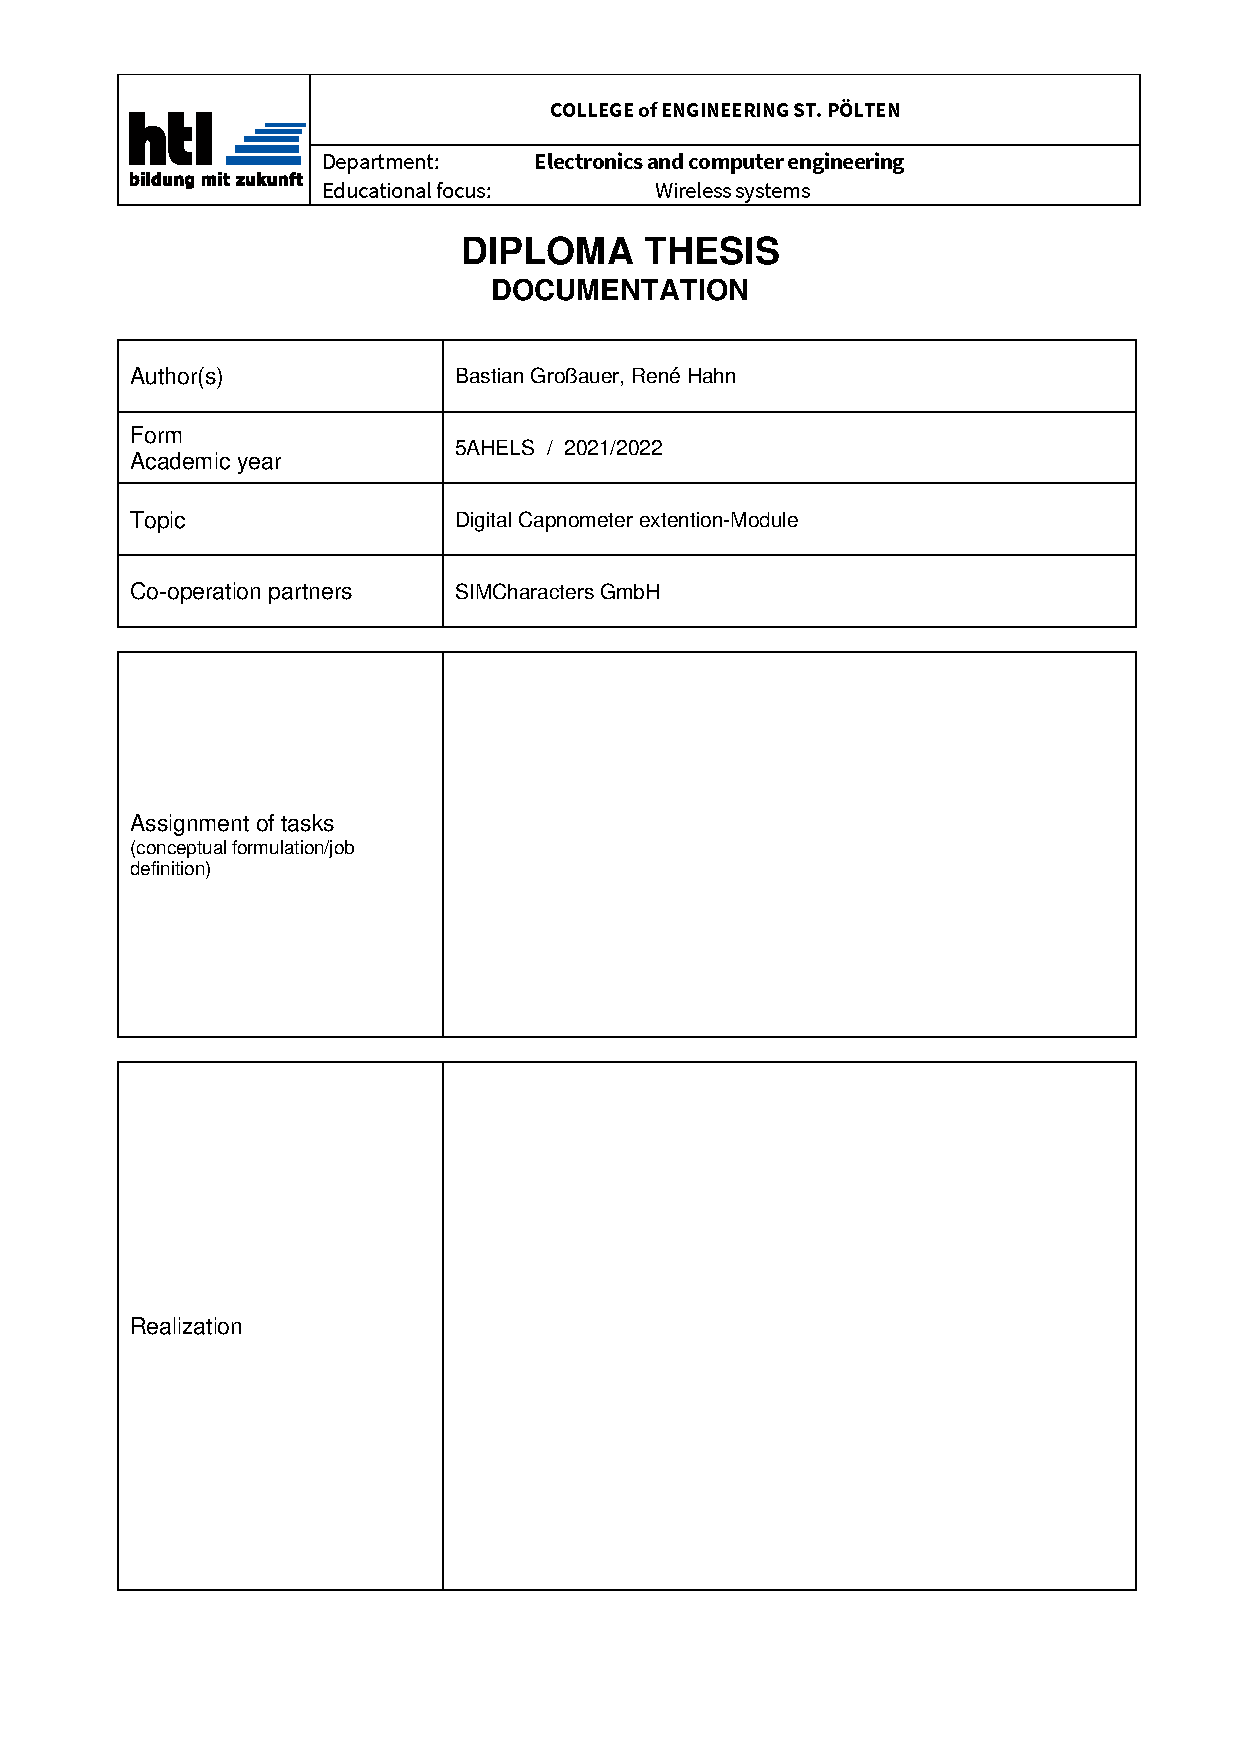
\includepdf[pages={1-2}]{./pdf/DA_3_CAPNO_nf.pdf}                                     % then export as pdf and add here

\clearpage
\thispagestyle{empty}
\hfill
\clearpage

\fancyhead{}
\clearpage


% --------------------------------------------- Acknoledgment -----------------------------------------------

\section*{Acknoledgement} 
\fancyfoot[RO,LE]{\thepage}   
\pagenumbering{Roman}                                                                     % set page count to roman numbers ONLY ON Table of content 
\setcounter{page}{1}

\fancyhead[RO,LE]{\textbf{Digital Capnometer Extention Module}\\\small{Acknoledgement}}   % change per new section


The overall goal of this ...

\clearpage


% ------------------------------------------- Table of Contents ---------------------------------------------

\fancyhead{}
\fancyhead[RO,LE]{\textbf{Digital Capnometer Extention Module}\\\small{Contents}}       % change small per new section
%                                                                                       % reseting page count for ToC
\tableofcontents

\clearpage


% ----------------------------------------------- Preamble --------------------------------------------------

\setcounter{section}{-1}
\section{Preamble}
\setcounter{section}{0}
\fancyhead[RO,LE]{\textbf{Digital Capnometer Extention Module}\\\small{Preamble}}       % change per new section
\fancyfoot[RO,LE]{Page \thepage}    
\pagenumbering{arabic}                                                                  % set page count to roman numbers ONLY ON Table of content 
\setcounter{page}{1}

The overall goal of this ...

\fancyfoot[C]{Bastian Großauer}                                                         % change to who wrote that page, per page 

\clearpage



% --------------------------------------------- Introduction ------------------------------------------------

\section{Introduction}
\fancyhead[RO,LE]{\textbf{Digital Capnometer Extention Module}\\\small{Introduction}}

The overall goal of this ...


\subsection{Current Situation}

Paul is a trainingssimulator for medicine students and doctors, who want to practice
an emergency case in neonatology.


\subsubsection{Pauls Problem without the Capnometer}

The objective was to create a module, that simulates a capnometer, while communicating
with Paul.


\subsection{Possible Approaches}

The objective was to create a module, that simulates a capnometer, while communicating
with Paul.


\subsubsection{Challenges}

The objective was to create a module, that simulates a capnometer, while communicating
with Paul.


\subsubsection{Display}

The objective was to create a module, that simulates a capnometer, while communicating
with Paul.


\paragraph{Problem Factors}

The objective was to create a module, that simulates a capnometer, while communicating
with Paul.

\fancyfoot[C]{René Hahn}

\clearpage


% --------------------------------------------- Specifications ------------------------------------------------

\section{Specifications}
\fancyhead[RO,LE]{\textbf{Digital Capnometer Extention Module}\\\small{Specifications}}

The overall goal of this ...


\subsection{Current Situation}

Paul is a trainingssimulator for medicine students and doctors, who want to practice
an emergency case in neonatology.


\subsubsection{Pauls Problem without the Capnometer}

The objective was to create a module, that simulates a capnometer, while communicating
with Paul.


\subsection{Possible Approaches}

The objective was to create a module, that simulates a capnometer, while communicating
with Paul.


\subsubsection{Challenges}

The objective was to create a module, that simulates a capnometer, while communicating
with Paul.


\subsubsection{Display}

The objective was to create a module, that simulates a capnometer, while communicating
with Paul.


\paragraph{Problem Factors}

The objective was to create a module, that simulates a capnometer, while communicating
with Paul.

\fancyfoot[C]{René Hahn}

\clearpage


% ----------------------------------------------- Concept --------------------------------------------------

\section{Concept}
\fancyhead[RO,LE]{\textbf{Digital Capnometer Extention Module}\\\small{Concept}}

The overall goal of this ...


\subsection{Current Situation}

Paul is a trainingssimulator for medicine students and doctors, who want to practice
an emergency case in neonatology.


\subsubsection{Pauls Problem without the Capnometer}

The objective was to create a module, that simulates a capnometer, while communicating
with Paul.


\subsection{Possible Approaches}

The objective was to create a module, that simulates a capnometer, while communicating
with Paul.


\subsubsection{Challenges}

The objective was to create a module, that simulates a capnometer, while communicating
with Paul.


\subsubsection{Display}

The objective was to create a module, that simulates a capnometer, while communicating
with Paul.


\paragraph{Problem Factors}

The objective was to create a module, that simulates a capnometer, while communicating
with Paul.

\fancyfoot[C]{René Hahn}

\clearpage

% ---------------------------------- Partition in Hardware and Software ------------------------------------
\section{Partition in Hardware and Software}
\fancyhead[RO,LE]{\textbf{Digital Capnometer Extention Module}\\\small{Partition in Hardware and Software}}

The overall goal of this ...


\subsection{Current Situation}

Paul is a trainingssimulator for medicine students and doctors, who want to practice
an emergency case in neonatology.


\subsubsection{Pauls Problem without the Capnometer}

The objective was to create a module, that simulates a capnometer, while communicating
with Paul.


\subsection{Possible Approaches}

The objective was to create a module, that simulates a capnometer, while communicating
with Paul.


\subsubsection{Challenges}

The objective was to create a module, that simulates a capnometer, while communicating
with Paul.


\subsubsection{Display}

The objective was to create a module, that simulates a capnometer, while communicating
with Paul.


\paragraph{Problem Factors}

The objective was to create a module, that simulates a capnometer, while communicating
with Paul.

\fancyfoot[C]{René Hahn}

\clearpage


% --------------------------------------------- Used Technologies ------------------------------------------------

\section{Used Technologies}
\fancyhead[RO,LE]{\textbf{Digital Capnometer Extention Module}\\\small{Used Technologies}}

The overall goal of this ...


\subsection{Current Situation}

Paul is a trainingssimulator for medicine students and doctors, who want to practice
an emergency case in neonatology.


\subsubsection{Pauls Problem without the Capnometer}

The objective was to create a module, that simulates a capnometer, while communicating
with Paul.


\subsection{Possible Approaches}

The objective was to create a module, that simulates a capnometer, while communicating
with Paul.


\subsubsection{Challenges}

The objective was to create a module, that simulates a capnometer, while communicating
with Paul.


\subsubsection{Display}

The objective was to create a module, that simulates a capnometer, while communicating
with Paul.


\paragraph{Problem Factors}

The objective was to create a module, that simulates a capnometer, while communicating
with Paul.

\fancyfoot[C]{René Hahn}

\clearpage


% --------------------------------------------- Research ------------------------------------------------

\section{Research}
\fancyhead[RO,LE]{\textbf{Digital Capnometer Extention Module}\\\small{Research}}

The overall goal of this ...


\subsection{Current Situation}

Paul is a trainingssimulator for medicine students and doctors, who want to practice
an emergency case in neonatology.


\subsubsection{Pauls Problem without the Capnometer}

The objective was to create a module, that simulates a capnometer, while communicating
with Paul.


\subsection{Possible Approaches}

The objective was to create a module, that simulates a capnometer, while communicating
with Paul.


\subsubsection{Challenges}

The objective was to create a module, that simulates a capnometer, while communicating
with Paul.


\subsubsection{Display}

The objective was to create a module, that simulates a capnometer, while communicating
with Paul.


\paragraph{Problem Factors}

The objective was to create a module, that simulates a capnometer, while communicating
with Paul.

\fancyfoot[C]{René Hahn}

\clearpage


% ------------------------------------------ Hardware Design -------------------------------------------

\section{Hardware Design}
\fancyhead[RO,LE]{\textbf{Digital Capnometer Extention Module}\\\small{Hardware Design}}

The overall goal of this ...


\subsection{Current Situation}

Paul is a trainingssimulator for medicine students and doctors, who want to practice
an emergency case in neonatology.


\subsubsection{Pauls Problem without the Capnometer}

The objective was to create a module, that simulates a capnometer, while communicating
with Paul.


\subsection{Possible Approaches}

The objective was to create a module, that simulates a capnometer, while communicating
with Paul.


\subsubsection{Challenges}

The objective was to create a module, that simulates a capnometer, while communicating
with Paul.


\subsubsection{Display}

The objective was to create a module, that simulates a capnometer, while communicating
with Paul.


\paragraph{Problem Factors}

The objective was to create a module, that simulates a capnometer, while communicating
with Paul.

\fancyfoot[C]{René Hahn}

\clearpage

% ------------------------------------------- Software Design -----------------------------------------------

\section{Software Design}
\fancyhead[RO,LE]{\textbf{Digital Capnometer Extention Module}\\\small{Software Design}}

The overall goal of this ...


\subsection{Current Situation}

Paul is a trainingssimulator for medicine students and doctors, who want to practice
an emergency case in neonatology.


\subsubsection{Pauls Problem without the Capnometer}

The objective was to create a module, that simulates a capnometer, while communicating
with Paul.


\subsection{Possible Approaches}

The objective was to create a module, that simulates a capnometer, while communicating
with Paul.


\subsubsection{Challenges}

The objective was to create a module, that simulates a capnometer, while communicating
with Paul.


\subsubsection{Display}

The objective was to create a module, that simulates a capnometer, while communicating
with Paul.


\paragraph{Problem Factors}

The objective was to create a module, that simulates a capnometer, while communicating
with Paul.

\fancyfoot[C]{René Hahn}

\clearpage


% ------------------------------------------------ Results ---------------------------------------------------
--
\section{Results}
\fancyhead[RO,LE]{\textbf{Digital Capnometer Extention Module}\\\small{Results}}

The overall goal of this ...


\subsection{Current Situation}

Paul is a trainingssimulator for medicine students and doctors, who want to practice
an emergency case in neonatology.


\subsubsection{Pauls Problem without the Capnometer}

The objective was to create a module, that simulates a capnometer, while communicating
with Paul.


\subsection{Possible Approaches}

The objective was to create a module, that simulates a capnometer, while communicating
with Paul.


\subsubsection{Challenges}

The objective was to create a module, that simulates a capnometer, while communicating
with Paul.


\subsubsection{Display}

The objective was to create a module, that simulates a capnometer, while communicating
with Paul.


\paragraph{Problem Factors}

The objective was to create a module, that simulates a capnometer, while communicating
with Paul.

\fancyfoot[C]{René Hahn}

\clearpage


% --------------------------------------------- Economical Part ------------------------------------------------

\section{Economical Part}
\fancyhead[RO,LE]{\textbf{Digital Capnometer Extention Module}\\\small{Economical Part}}

The overall goal of this ...


\subsection{Current Situation}

Paul is a trainingssimulator for medicine students and doctors, who want to practice
an emergency case in neonatology.


\subsubsection{Pauls Problem without the Capnometer}

The objective was to create a module, that simulates a capnometer, while communicating
with Paul.


\subsection{Possible Approaches}

The objective was to create a module, that simulates a capnometer, while communicating
with Paul.


\subsubsection{Challenges}

The objective was to create a module, that simulates a capnometer, while communicating
with Paul.


\subsubsection{Display}

The objective was to create a module, that simulates a capnometer, while communicating
with Paul.


\paragraph{Problem Factors}

The objective was to create a module, that simulates a capnometer, while communicating
with Paul.

\fancyfoot[C]{René Hahn}

\clearpage

% ------------------------------------------ Project Management ---------------------------------------------

\section{Project Management}
\fancyhead[RO,LE]{\textbf{Digital Capnometer Extention Module}\\\small{Project Management}}

The overall goal of this ...


\subsection{Current Situation}

Paul is a trainingssimulator for medicine students and doctors, who want to practice
an emergency case in neonatology.


\subsubsection{Pauls Problem without the Capnometer}

The objective was to create a module, that simulates a capnometer, while communicating
with Paul.


\subsection{Possible Approaches}

The objective was to create a module, that simulates a capnometer, while communicating
with Paul.


\subsubsection{Challenges}

The objective was to create a module, that simulates a capnometer, while communicating
with Paul.


\subsubsection{Display}

The objective was to create a module, that simulates a capnometer, while communicating
with Paul.


\paragraph{Problem Factors}

The objective was to create a module, that simulates a capnometer, while communicating
with Paul.

\fancyfoot[C]{René Hahn}

\clearpage


% ----------------------------------------------- Appendix -------------------------------------------------


\section{Appendix}
\fancyhead[RO,LE]{\textbf{Digital Capnometer Extention Module}\\\small{Appendix}}

The overall goal of this ...


\subsection{Milestones}

One part of project management is the milestone setting, because ...


\subsection{Internal Devision of Duties}

Bastian Großauer is in charge of the Hardware Design...

\subsection{Schedule}

The project was scheduled as ...


\subsection{Contact with the Projectpartner SIMCharacters GmbH}

Initially, an email was sent to Michel Haller if this company could offer a ...


\subsection{Diploma Seminars}

In the following pages the diploma seminars are visualized ...

\fancyfoot[C]{René Hahn}

\clearpage

\end{document}
